% !TeX spellcheck = de_DE
\documentclass[.../Dokumentation.tex]{subfiles}
\begin{document}
\subsection{Ergebnis}\label{sec-ita3-result}
Obgleich die gewünschten Freiräume im Fahrzeuginneren erhalten werden konnten, 
indem ohne Stützmaterial gedruckt wurde, ergaben sich hierdurch neue Probleme.
Da nun gar keine Stützen mehr gesetzt wurden, konnten einige Außenflächen wie 
beispielsweise an der Motorhaube nicht zufriedenstellend gedruckt werden.
Auch die Unterseite des Fahrzeugs ist betroffen, wenn auch weniger stark.
Beide Stellen sind in Abbildung \ref{fig-hood-no-support} zu sehen.
Des Weiteren wurde deutlich, dass sich durch Zusammenspiel aus modellierten 
Maßen und den vom Drucker erreichbaren Präzisionsintervallen Aussparungen 
ergaben, die kleiner als geplant produziert wurden.
Hiervon betroffen waren die Scheinwerfer und der Hall-Sensor.
\begin{figure}[H]
\begin{center}
    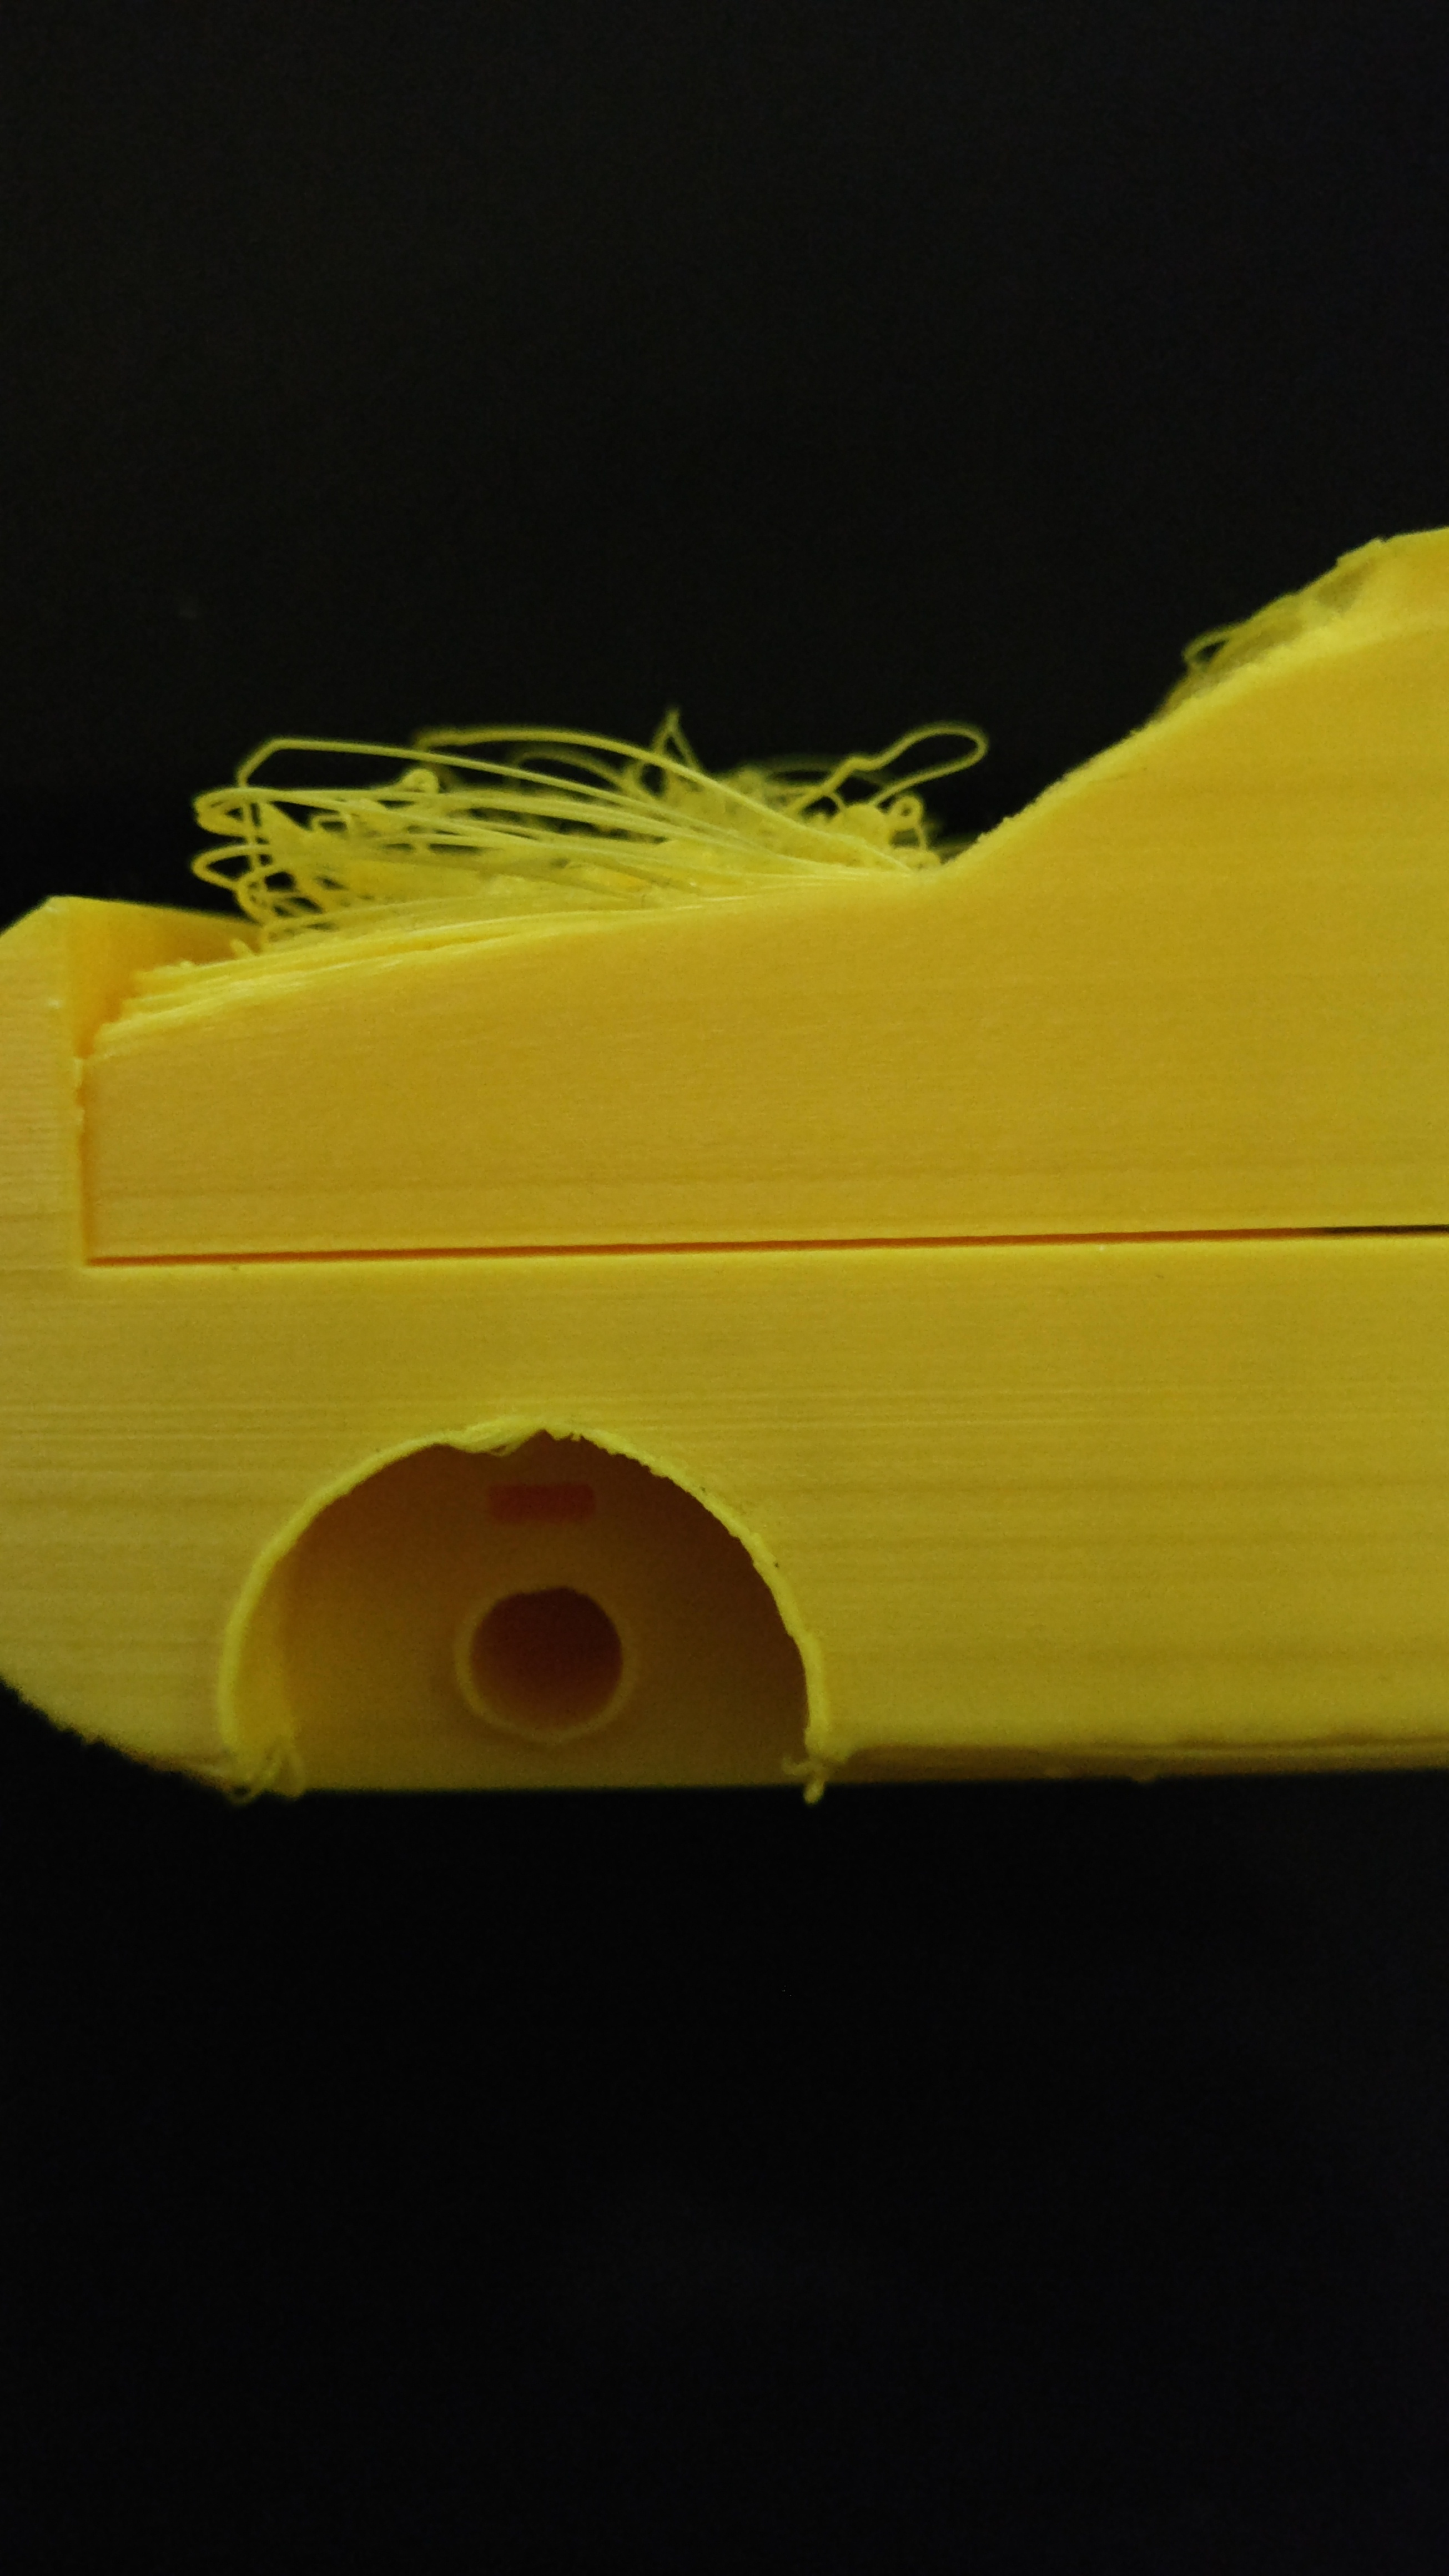
\includegraphics[
        width=0.5\linewidth,
    ]{imgs/hood_without_support.jpg}
    \caption{Probleme beim Druck ohne Stützmaterial}
    \label{fig-hood-no-support}
\end{center}
\end{figure}
\noindent
Während der neue Ansatz zur Visualisierung konzeptionell durchaus 
vielversprechend schien, so konnte mit den in Abbildung \ref{fig-tree-in-box} 
gezeigten Bauteilen nicht fortgefahren werden. Sowohl die Box als auch der Baum selbst wurden aus Holzplatten von 3mm 
Stärke ausgeschnitten. Insbesondere der Baum war auf Grund der Kombination 
aus filigranen Blättern und Ästen mit dem zu schwach gewählten Material nicht 
weiter zu verwenden. Bereits durch den Transport aus den Räumlichkeiten 
des \textit{FabLab} verlor er eine Vielzahl an Blättern. Weiter hätten die Äste 
geteilt werden müssen, um das in \ref{sec-ita3-visualization} vorgestellte 
Konzept umzusetzen. Die Box selbst wurde als zu instabil beurteilt, als dass sie die Montage der Motoren und des Raspberry Pi hätte verkraften können.\\
Die Fahrzeugschaltung wurde um einen \textit{Step-Up Boost-Converter} erweitert. Hierdurch ist der reibungslose Betrieb auch bei Stromversorgung durch den Akku gewährleistet. Des Weiteren wurde auf Basis der Hardware der Visualisierung eine Schaltung erstellt und entsprechender Programmcode implementiert. Die Kommunikation zwischen den einzelnen Komponenten ist ab diesem Zeitpunkt funktionsfähig, sodass Verschmutzungswerte ausgewertet und dargestellt werden können.
\end{document}